\documentclass[letterpaper]{article}
\usepackage[submission]{aaai2027}
\usepackage[hyphens]{url}
\usepackage{graphicx}
\urlstyle{rm}
\def\UrlFont{\rm}
\usepackage{natbib}
\usepackage{caption}
\usepackage{booktabs}
\usepackage{amsmath}
\frenchspacing

\pdfinfo{
/TemplateVersion (2027.1)
}

\setcounter{secnumdepth}{0}

\title{Updating the World Is Not Rebinding the Target:\\
Temporal Referent Integrity in Tool-Using Agents}
\author{Anonymous Submission}
\affiliations{}

\begin{document}
\maketitle

\begin{abstract}
Refreshing external state does not by itself authorize a tool-using agent to change the entity
denoted by an earlier reference. We formalize this post-binding problem as \emph{temporal
referent integrity} (TRI), separating world-state updates from referent-transition authorization.
We construct Preserve/Reevaluate contrasts that hold both states, selector, and action fixed while
varying when the target is resolved. On a frozen 160-task diagnostic, a Generic Structured Ledger
reaches 64.4\%/71.9\% with Qwen3.5/GLM-5.1, whereas pre-refresh Compile-then-act (CTA)
reaches 95.0\%/96.2\%; unconditional locking and reevaluation each reach 60.0\% and fail
complementary cases. A disclosed post-hoc benchmark-aware rule reaches 92.5\%, narrowing the
algorithmic claim to executable authorization rather than method complexity. In a separately
frozen 240-task replication, Generic frequently substitutes
the refreshed winner after a correct initial binding, while an explicit pre-refresh commitment
policy exhibits no such conditional drift; replay converts these substitutions into wrong-entity
SQLite writes. Human judgments support Preserve/Reevaluate, while public benchmark audits find
few native opportunities to measure it. TRI is a controlled, model- and controller-conditional
diagnosis supporting executable transition authorization as a design principle, not a
prevalence or general-safety claim.
\end{abstract}

\section{Introduction}

Consider two requests issued before the same mailbox refresh:

\begin{quote}
\small
(1) ``Choose the highest-priority unread email now. Refresh the mailbox, then reply to it.''

(2) ``Refresh the mailbox first. Then choose the highest-priority unread email and reply.''
\end{quote}

Suppose email A is highest priority before refresh and email B afterward. The environment
transition is identical, but the correct target differs. Request (1) establishes A as an
identity commitment; request (2) deliberately leaves a description to be evaluated in the
new state. Acting on B in (1) is not stale-state correction. It is a wrong-entity action.

This distinction is easy to lose in LLM agent controllers. A controller may preserve the
entire transcript, append the latest observation, and ask a downstream model to act. All
facts remain available, yet the model can silently apply the old selector to the new state.
Conversely, always retaining an old ID breaks genuinely dynamic references. Reliable tool
use therefore needs \emph{selective invariance}: world facts should update while some target
denotations remain fixed, others are reevaluated, and invalid commitments follow an explicit
fallback policy.

We call this property \emph{temporal referent integrity} (TRI). TRI is not ordinary entity
memory. Remembering an ID does not say whether that ID is a committed referent or merely the
previous output of a dynamic selector. Nor does existence imply action validity: an email may
remain present but cease to be replyable. Finally, the selector that established identity is
not necessarily a persistent validity predicate. A branch chosen because it was default can
stop being default while remaining the correct branch on which to run checks.

Figure~\ref{fig:mechanism} summarizes the problem and our controller. A Generic Structured
Ledger records identity, facts, selector, and action preconditions, while leaving the actor to
infer how those fields interact across refresh. Minimal Compile-then-act (CTA) first records
binding time and identity. Its typed Lifecycle-Gated extension adds validity and fallback state;
a deterministic gate enforces preserved identities while an actor resolves dynamic branches.

\begin{figure*}[t]
\centering
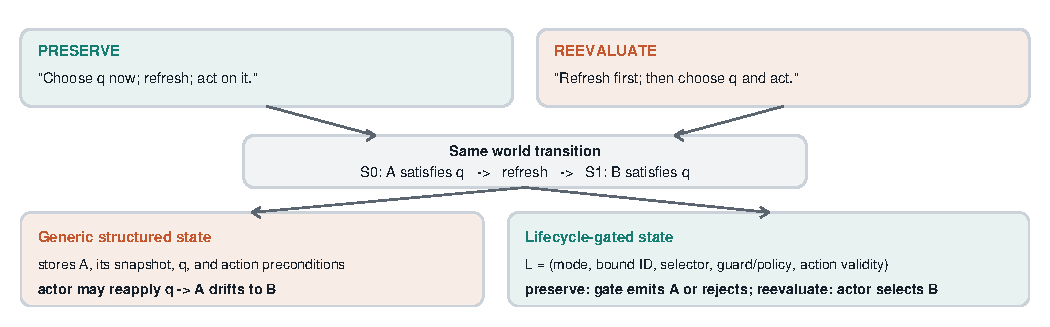
\includegraphics[width=0.98\textwidth]{Figures/tri_v3_mechanism.pdf}
\caption{The same state transition requires different targets depending on discourse. Generic
structured state preserves facts but leaves the interaction between identity and selector
implicit. Lifecycle state makes the permitted denotation update executable.}
\label{fig:mechanism}
\end{figure*}

Our contributions are fourfold:
\begin{itemize}
    \item We isolate post-binding referent-transition authorization: after a target is correctly
    resolved, changed world evidence need not authorize changing its identity.
    \item We introduce clustered Preserve/Reevaluate diagnostics whose matched members require
    opposite targets under the same world transition, with pre-specified cluster statistics.
    \item Under controlled conditions, tested controllers sometimes replace a correctly bound,
    still-valid target with the refreshed selector winner; deterministic replay converts these
    substitutions into wrong-entity mutations.
    \item CTA, typed lifecycle state with gating, and a disclosed benchmark-aware rule instantiate
    one implementation-independent separation principle. Public audits and negative stress tests
    bound it: current benchmarks rarely expose strict opportunities, and scalar contracts do not
    compose automatically.
\end{itemize}

\section{Related Work}

\paragraph{Reference, binding, and memory.}
Discourse theories distinguish referents from changing descriptions and salience
\cite{kamp1993discourse,grosz1995centering}; coreference work recovers textual identity links
\cite{lee2017coreference,joshi2020spanbert,dasigi2019quoref}. Entity Binding Failures studies
wrong initial tool arguments \cite{babu2026entitybinding}; TRI instead conditions on correct
$bind(r,S_0)$ and asks whether $S_1$ licenses a transition. Agent memory and entity tracking retain
facts or traces \cite{tang2026entitytracking,zhang2024memorysurvey,packer2023memgpt,
sumers2024coala,yao2023react};
correctly tracking the new selector winner still does not authorize acting on it. Temporal
Blindness asks when time should trigger a new observation \cite{cheng2026temporalblindness}; TRI
asks what that observation may revise. Evolving-environment benchmarks study belief and memory
adaptation \cite{ji2026clawarena,xu2026evoarena}; TRI studies the propagation boundary from
belief updates to an already resolved action referent.

\paragraph{Binding Drift.}
The closest neighbor studies silent entity replacement in multi-step workflows and evaluates
locking and re-verification \cite{indukuri2026bindingdrift}. TRI substantially overlaps its Preserve
branch but also includes authorized Reevaluate cases: ``choose now, refresh, act'' and ``refresh,
then choose'' require opposite targets under the same transition. We reproduce its deterministic
offline harness, but its oracle re-verifier reads a gold target; its Entity Lock corresponds to
our Always-Lock extreme. Its LLM-based self/cross re-verifiers resolve the original step-1 referent
and target initial binding or propagation; they do not expose a separate user-authorized deferred
query. TRI instead isolates a complementary variable that preserve-only evaluation cannot
identify: whether post-update re-resolution is user-authorized. Initial-binding correctness and post-update transition authorization
are orthogonal: TRI conditions on the former to isolate the latter. Our author adaptation supplies
the complete temporal instruction rather than Binding Drift's short referent interface; it is not
an official LLM-sweep reproduction. Because it sees $S_1$ but neither $S_0$ nor the resolved old
ID, we treat it as an interface audit rather than an information-matched performance baseline.

\paragraph{Tool agents and executable constraints.}
Tool-use benchmarks cover APIs, web environments, and stateful interaction
\cite{schick2023toolformer,li2023apibank,qin2024toolllm,patil2023gorilla,
liu2024agentbench,zhou2024webarena,lu2025toolsandbox,trivedi2024appworld,
yao2024taubench,barres2025tau2,sierra2026tau3,ruan2024toolemu}.
Their gold does not label post-binding
Preserve/Reevaluate opportunities. LedgerAgent and Bounded Autonomy add typed state or action
contracts \cite{uddin2026ledgeragent,sohail2026bounded}; action validity still cannot determine
which valid entity discourse authorized. Structured generation can enforce syntax
\cite{beurer2023lmql,willard2023guided,khattab2024dspy}, while our clustered minimal pairs
follow diagnostic and contrast-set methodology \cite{ribeiro2020checklist,gardner2020contrast}.
Complementary semantic conditions have similarly exposed one-sided LLM heuristics and correction
trade-offs in aspectual NLI \cite{ma2026imperfective}; TRI applies the diagnostic logic to
post-binding control and executed actions, not lexical aspect or static entailment.

\section{Problem Formulation: Temporal Referent Integrity}

Let $H_t$ be interaction history, $S_t$ world state, $r$ an action-target reference, and $q_r$
its selector. Referential control state is either an unresolved query $C_t(r)=U(q_r)$ or a bound
commitment $C_t(r)=B(e)$. Language and history induce a transition authorization
$\Gamma_{t+1}(r,e\!\rightarrow\!e')$; a world update alone does not:
\begin{equation}
\begin{aligned}
S_t\ne S_{t+1}&\;\not\Rightarrow\;C_t(r)\ne C_{t+1}(r),\\
B(e)\to B(e'),\ e'\ne e&\;\Rightarrow\;\Gamma_{t+1}(r,e\to e').
\end{aligned}
\end{equation}
Thus a selector can be evaluated to establish $B(q_r(S_0))$, preserved across refresh, or left
as $U(q_r)$ for authorized evaluation in $S_1$. Returning from $B(e)$ to query evaluation requires
authorization; a refreshed selector winner is evidence about the world, not such authorization.

\paragraph{State--authorization separation.}
Updating $S_t$ alone does not mutate a bound $C_t(r)$. History may contain enough discourse
evidence to infer the permitted transition, but information availability does not imply that a
model-mediated controller will operationalize or enforce it reliably. TRI concerns the control
effect of an update, not whether the new world state is known correctly. Explicit authorization
state is one implementation; the formal requirement is access to a discourse-sensitive transition
decision, not a particular field or serialization.

For execution, $V_a(e,S)$ denotes action-relative validity and $\pi$ an invalid-target policy.
Our lifecycle record $L=(m,e,q,g,V_a,\pi)$ is one implementation of this state machine, not the
definition of TRI. TRI-v3 uses $m\in\{\textsc{Preserve},\textsc{Reevaluate}\}$; TRI-v4 adds a
conditional guard $g$.

For the scalar policies evaluated here, the execution branches are
\begin{align}
\textsc{Preserve},\;V_a(e,S_1) &\Rightarrow e, \\
\textsc{Preserve},\;\neg V_a(e,S_1),\;\pi=\textsc{Reject} &\Rightarrow \bot, \\
\textsc{Reevaluate} &\Rightarrow q(S_1), \\
\textsc{Conditional},\;g(e,q,S_1) &\Rightarrow e, \\
\textsc{Conditional},\;\neg g(e,q,S_1) &\Rightarrow q(S_1).
\end{align}
An invalid preserved entity remains $B(e)$ even when execution returns $\bot$.
Likewise, $q$ establishes identity under Preserve but remains unresolved under Reevaluate;
action validity never authorizes substituting a different valid entity. Full history may contain
all necessary facts while leaving this relationship computationally implicit; a deterministic
guarantee additionally requires enforcement at the mutation boundary. TRI-v4 distinguishes
$g_{\mathrm{act}}=V_a(e,S_1)$ from $g_{\mathrm{sel}}=[q(S_1)=e]$.

\paragraph{Proposition (mode-blind policy impossibility).}
Consider a Preserve/Reevaluate minimal pair with identical $S_0$, $S_1$, $q$, and $a$, where
$e=q(S_0)$, $e'=q(S_1)$, and $e\ne e'$. The authorized targets are $e$ and $e'$, respectively.
Any deterministic post-refresh policy of the form $f(e,q,S_1,a)$, containing neither the
original history nor a compiled transition authorization,
receives the same inputs for both tasks and must return the same target; it is therefore wrong
on at least one member. Always-Lock and
Always-Reevaluate instantiate the two complementary extremes measured in our policy controls.
This establishes the need for a discourse-sensitive transition decision, not the necessity of
our particular serialization. It is an identifiability result for the diagnostic variable, not a
lower bound on model, algorithm, or representation complexity.

\paragraph{Authorization invariant (conditional guarantee).}
If $L$ is correct, IDs are stable, selector/guard evaluation is correct, and the executor follows
the branches above, every emitted target is referentially authorized; enforcing $V_a$ additionally
makes each executed mutation action-valid. The guarantee ends at compilation: a wrong but valid
ID, identity migration, or an incomplete action schema can still pass.

\paragraph{Outcomes.}
We separately report exact target/final state, wrong-entity writes, invalid attempts, and
unnecessary rejection; always rejecting avoids writes but fails every actionable task.

\section{Realizing Transition Authorization}

The claim has three levels. The design principle is to make transition authorization executable.
Minimal CTA tests it through pre-refresh commitment compilation, emitting binding time, selector,
and a bound ID. The typed Lifecycle implementation adds an auditable validity/fallback contract,
and Lifecycle-Gated enforces that contract at mutation time. It additionally emits
\begin{quote}
\small\ttfamily
reference\_mode; bound\_target\_id; selector; invalidity\_policy.
\end{quote}
Both compilers use discourse order: ``identify, refresh, act on it'' preserves identity even
without words such as ``same,'' while ``refresh before deciding'' reevaluates. It resolves a
concrete bound ID only for preserved references.

The executor then refreshes the environment. If the compiled mode is \textsc{Preserve}, a
deterministic gate checks the bound entity against action preconditions. The gate emits the
bound ID when valid, returns $\bot$ under a reject policy, or invokes selector resolution only
when the compiled fallback authorizes it. If the mode is \textsc{Reevaluate}, the LLM actor
selects from $S_1$. Thus a preserved commitment is a controller constraint, not advice that a
second model may reinterpret. The gated Preserve branch needs one model call rather than two.

TRI-v4 generalizes the record with \texttt{guard\_type} and
\texttt{fallback\_policy}. The action-validity guard can be enforced deterministically. A
selector-match guard is evaluated by the actor because the current prototype compiles natural
language selectors but does not execute them as a general symbolic query language. This design
choice exposes selector grounding as a measurable stage rather than using gold selector fields.

The complete controller procedure and model-facing interfaces are provided in the supplement.
Gold targets and benchmark selector fields are never provided to the compiler or actor.

\paragraph{Information fairness.}
Compilers see the instruction, $S_0$, action schema, and planned refresh, never gold targets or
generator selector fields. Generic retains the instruction, selected ID, snapshot, selector,
action, and preconditions for its second-call actor. CTA, Lifecycle-free, and Generic each use
two calls; Lifecycle-Gated skips the actor for a valid Preserve branch. Full prompts, interfaces,
and executor-level oracle checks are supplementary.

\section{Experimental Setup}

\paragraph{Controlled task construction.}
Each domain specification defines an entity table, a natural-language selector, its ranking or
Boolean criterion, an action, and explicit action preconditions. The generator first evaluates
the selector on $S_0$ to obtain $e_0$, applies a controlled transition, and evaluates it on
$S_1$ to obtain $e_1$. A language template determines whether the action target is $e_0$,
$e_1$, $\bot$, or a conditionally guarded choice. Paired tasks share the domain, both states,
selector, action, and schema; only discourse order and anaphoric language change. This prevents
domain difficulty or target frequency from explaining the preserve/reevaluate contrast.

The referential core is a crossed diagnostic: authorization is \textsc{Preserve} or
\textsc{Reevaluate}, while the refreshed selector winner is unchanged (Stable) or changed
(Flip/name collision). Stable controls test ordinary execution without a target conflict;
changed-winner pairs require opposite targets under identical states. Remove and Invalidate form
a separate execution-policy slice because anchored items may require rejection rather than an ID.

The five transition types serve different diagnostic roles. \emph{Flip} changes which valid
entity wins the selector. \emph{Stable} leaves the winner unchanged and detects controllers
that overreact to any refresh. \emph{Remove} deletes the pre-refresh entity. \emph{Invalidate}
keeps its ID present while changing an action-precondition field, separating existence from
validity. \emph{Name collision} gives another entity the same display label while changing the
selector winner, testing whether controllers preserve stable identity rather than surface
aliases. Across anchored and dynamic language, these updates create matched cases where naive
``always old'' and ``always new'' policies have complementary failures.

\paragraph{Blind human construct validation.}
One independent volunteer naturally rewrote 50 sampled scalar instructions. Three other
volunteers, uninvolved in TRI design, independently labeled 100 randomized original/rewrite
items using opaque IDs without condition metadata or gold answers. They selected an entity,
\textsc{Reject}, or \textsc{Clarify}; confidence was optional. We report majority--gold
alignment, unanimous and pairwise agreement, Fleiss' $\kappa$, nominal Krippendorff's $\alpha$,
and a consensus-only sensitivity analysis. Conditional, collection, and nested cases were not
included in this human study.

Stage and write-consequence reports use a frozen mechanism-oriented error taxonomy, detailed
in the supplement, that separates temporal rebinding, premature binding, invalid processing,
unnecessary rejection, and selector-grounding errors.

\paragraph{Symmetric evaluation and component audit.}
Figure~\ref{fig:calibration} visualizes the frozen v3 changed-winner core. Generic validity gating,
an untyped pre-refresh plan, Lifecycle-free execution, and exact historical Compile-then-act
were post-primary audits; they do not replace the pre-specified Generic-versus-Lifecycle-Gated
estimand. A later handcrafted rule is an explicitly post-hoc strong baseline. The full component
table is supplementary; together these audits determine how narrowly the comparison can be read.

\begin{figure}[t]
\centering
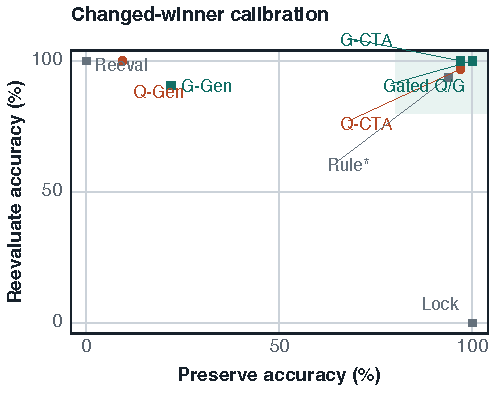
\includegraphics[width=\columnwidth]{Figures/tri_authorization_tradeoff_compact.pdf}
\caption{Preserve versus Reevaluate accuracy on 32 matched v3 changed-winner pairs; label numbers
are PairAcc. Unconditional controls occupy opposite corners. Generic succeeds mainly on
Reevaluate, whereas joint success lies in the upper right. Rule v2 is post-hoc; the reject-policy
slice is excluded.}
\label{fig:calibration}
\end{figure}

\paragraph{TRI-v3 language clusters.}
The primary test contains 160 tasks formed from 20 frozen language-template clusters,
four reference styles, and eight domains per template. Within each style, flip, stable, remove,
invalidate, and name-collision updates are balanced. The pre-specified statistic resamples
whole template clusters with 10,000 bootstrap samples; task-level McNemar is secondary. Before
any model call, we froze the data, runner, hashes, inference settings, and rule that prompts
would not change after output inspection.

\paragraph{Schema transfer under shared language templates and guarded policies.}
An 80-task transfer set crosses the same 20 template clusters with four new domains:
projects, expenses, inventory, and cloud deployments. These introduce new IDs, fields,
selectors, actions, and action preconditions. TRI-v4 separately freezes 40 conditional tasks,
ten template clusters, and the two guards $g_{\mathrm{act}}$ and $g_{\mathrm{sel}}$. Every
guard--update--domain combination occurs once. TRI-v4 is a secondary extension, not part of
the pre-specified v3 primary comparison.

\paragraph{Direct-neighbor baseline.}
Generic Structured Ledger uses two calls. Its compiler stores the initial selected ID, complete
entity snapshot, selector, requested action, and action preconditions, but omits reference mode
and invalidity policy. Its actor still receives the original instruction, ledger, $S_1$, and
action schema. It is therefore not an information-deletion baseline: the comparison asks
whether structured facts suffice without discourse commitment semantics.

The historical Compile-then-act prompt is rerun unchanged on the v3 language set.
Its cluster interval overlaps lifecycle-free execution for both
models, consistent with pre-refresh compilation, rather than tuple serialization or deterministic
gating alone, being the leading explanation. Because it emits binding time and a bound ID,
it also serves as the simple mode-classifier-plus-ID-lock analogue for scalar cases. The typed contract contributes an auditable
interface for validity and fallback; the gate is a small enforcement layer, not the principal
source of accuracy. A matched free-form pre-refresh planner reaches only 81.2\% for Qwen and
70.6\% for GLM, so moving computation before refresh is not alone sufficient; nevertheless,
the strong historical predecessor prevents us from claiming that the full tuple is empirically
necessary for scalar tasks.

For a direct policy contrast, we also evaluate two deterministic extremes without model calls.
Always-Lock + validity retains the $S_0$ ID and rejects it only when the refreshed action
preconditions fail; Always-Reevaluate discards the binding and applies $q$ to $S_1$. These are
conceptual controls rather than implementations of the Binding Drift baselines. On the frozen
160-task inventory both reach 96/160 (60.0\%), but their mode slices are complementary:
Always-Lock reaches 80/80 anchored and 16/80 dynamic, whereas Always-Reevaluate reaches
16/80 anchored and 80/80 dynamic. The contrast is a diagnostic of selective authorization,
not evidence that either unconditional policy is a competitive agent controller.

\paragraph{Model-facing SQLite trajectories.}
We freeze a 40-task subset covering all 20 templates, eight domains, both modes, and all update
types. The runtime queries an in-memory SQLite database, gives returned rows to the compiler,
replaces the database state during refresh, obtains a target from the gate or actor, and executes
\texttt{UPDATE} through a mutation tool that enforces action preconditions. We inspect final
database state, wrong writes, invalid attempts, and collateral modifications. Query and required
refresh order are controller-orchestrated; this is a focused execution test, not a fully
autonomous external benchmark.

\paragraph{Models, inference, and auditing.}
We use Qwen3.5-122B-A10B and GLM-5.1 through the same OpenAI-compatible API at temperature zero,
with thinking disabled and a 1,200-token output cap. A post-primary robustness replication uses
DeepSeek-V4-Pro with the same settings. Balanced smoke tests gate each expansion.
Final reports verify expected task IDs, duplicates, status, request attempts, and retries. All
reported v3/v4 full files are complete and contain zero API errors and zero retries. API failures
would be reported separately rather than interpreted as model behavior.

\paragraph{Statistical estimands.}
The primary estimand is Lifecycle-Gated minus Generic Structured Ledger accuracy on the Qwen
language-cluster set. We resample its 20 complete template clusters rather than treating 160
templated rows as independent. The same cluster bootstrap is reported for replication and
transfer sets; each interval uses 10,000 samples and a fixed recorded seed. Template-macro and
task accuracy coincide in the balanced sets, but both are retained in machine-readable reports.
For $N$ complete matched pairs, $\mathrm{PairAcc}=N^{-1}\sum_i
\mathbf{1}[\hat y_i^P=y_i^P\wedge\hat y_i^R=y_i^R]$; Preserve and Reevaluate marginal accuracy
are reported alongside it to reveal one-sided policies. Conditional drift is estimated only after
a correct observable initial binding when the old target remains valid and the winner changes.
Exact paired McNemar tests use task-level discordance and are secondary. Wilson intervals
describe individual proportions. Slices by binding, explicitness, update, and domain are
mechanism analyses rather than additional confirmatory hypotheses; we do not use them to select
the primary claim.

\paragraph{Reproducible run discipline.}
Frozen data, protocols, runners, and smoke subsets have recorded SHA-256 hashes. Reports retain
raw outputs, attempts, retries, stage errors, and SQLite traces; interrupted rows are auditable by
ID. The anonymous artifact maps every main-table value to a raw run and report script, includes
the human-analysis code and de-identified responses, and excludes API keys and private
coordination files. Post-primary audits are labeled as such.

\section{Results}

\subsection{Primary and Transfer Results}

\begin{table*}[t]
\centering
\small
\begin{tabular}{llrrrrr}
\toprule
Benchmark & Model & Generic E2E & CTA E2E & Lifecycle E2E & $\Delta$ & Cluster 95\% CI \\
\midrule
Language clusters (primary) & Qwen3.5 & 64.4 & 95.0 & 98.1 & +33.8 & [+18.1, +50.0] \\
Language clusters & GLM-5.1 & 71.9 & 96.2 & 100.0 & +28.1 & [+18.1, +38.1] \\
Core replication (new states) & Qwen3.5 & 47.5 & 70.8 & 71.2 & +23.8 & [+16.2, +31.2] \\
Core replication (new states) & GLM-5.1 & 70.0 & 94.2 & 97.1 & +27.1 & [+22.1, +32.1] \\
Schema transfer (shared templates) & Qwen3.5 & 46.2 & -- & 82.5 & +36.2 & [+25.0, +47.5] \\
Model-facing SQLite & Qwen3.5 & 67.5 & -- & 100.0 & +32.5 & [+15.0, +50.0] \\
Model-facing SQLite & GLM-5.1 & 65.0 & -- & 100.0 & +35.0 & [+17.5, +52.5] \\
Guarded conditional policies & Qwen3.5 & 52.5 & -- & 85.0 & +32.5 & [+15.0, +52.5] \\
\bottomrule
\end{tabular}
\caption{End-to-end (E2E) authorized-target accuracy (\%); SQLite rows instead use final
database-state success. These totals are not initial-binding accuracy or conditional TRI.
CTA is shown where run on the identical inventory; $\Delta$ is Lifecycle/Guarded minus Generic.
Intervals resample complete template or state-instance clusters.}
\label{tab:main}
\end{table*}

\paragraph{RQ1: Transition authorization is identifiable.}
Figure~\ref{fig:calibration} summarizes the symmetric test. Each matched pair holds $S_0,S_1,q,a$,
and the update fixed while changing whether resolution is
authorized before or after refresh. Stable leaves the winner unchanged; Flip changes it; name
collision gives old and new stable IDs the same display name. On 32 v3 changed-winner pairs,
PairAcc is 0/32 for both unconditional extremes, 3/32 and 7/32 for Qwen/GLM Generic, 30/32
and 31/32 for CTA, 32/32 for Gated, and 28/32 for the post-hoc rule. Stable is 16/16.
Thus aggregate accuracy cannot replace the symmetric test; full v3/v7 ITT tables are supplementary.
On 80 v7 changed-winner pairs, Generic obtains 7/15/17 for Qwen/GLM/DeepSeek, versus
31/66/64 for CTA and 60 for model-independent Rule v2; Gated obtains 40/73 for Qwen/GLM.
The weak Qwen CTA cell precludes a universal implementation claim while preserving the contrast.

\paragraph{RQ2: Tested controllers violate TRI after correct binding.}
Table~\ref{tab:main} shows the same behavioral contrast across models.
On the primary language-cluster test, Generic Structured Ledger reaches 64.4\% for Qwen and
71.9\% for GLM, despite carrying identity, facts, selector, preconditions, and the original
instruction; Lifecycle-Gated reaches 98.1\% and 100.0\%. Anchored accuracy rises from
33.8/56.2\% to 100.0/100.0\%, while dynamic performance is also retained. Paired tests and
complete mode slices are supplementary; the gain is not explained by always preserving old IDs.

Generic fails most when a valid bound entity no longer wins the selector. Conditioning on its
stored \texttt{selected\_entity\_id} being correct, Qwen drifts on 15/16 anchored flips and 14/16
name collisions; GLM drifts on 3/16 and 7/16, while Stable controls show none. This directionality
rules out random target error as a complete explanation.

The separately frozen v7 replication contains 240 core tasks over ten unseen schemas and 40
state instances; every old target remains present and action-valid. After a correct initial
binding, Generic selects exactly the distinct refreshed winner on 43/72 Qwen and 38/80 GLM
changed-winner opportunities, versus zero for matched CTA/Gated. A later DeepSeek run finds
59/79 versus 0/70 for Generic/CTA. SQLite replay turns every one of these 43, 38, and 59
substitutions into a wrong-entity write. The denominator excludes initial-ID, missing-ID,
action-invalid, API, and parse failures; Stable errors and all non-core writes remain separate.
Generic initial binding is correct on 107/120 Qwen, 120/120 GLM, and 119/120 DeepSeek anchored
rows; conditional drift intervals are [46.5,72.4], [35.0,61.3], and [62.5,86.1] percent.

\paragraph{A frozen write trace.}
In Qwen task \path{tri-v7-core-reminders-s1-explicit_anchor-name_collision}, Generic correctly
records initial winner \texttt{REM-1A}. After reload, valid \texttt{REM-1A} remains, but
\texttt{REM-1B} becomes earliest and shares display ``Renewal.'' The actor targets
\texttt{REM-1B}; SQLite records \texttt{wrong\_entity\_write}. CTA targets authorized
\texttt{REM-1A}. Raw outputs and the database trace are indexed in the supplement.

Leave-domain/template-out analyses retain a positive CTA--Generic E2E difference, and six
temperature-zero repeat cells retain its sign; incomplete task-level unanimity keeps the claim
aggregate and controller-conditional. We distinguish E2E, initial binding, conditional TRI, and
executed wrong-write denominators throughout.

\paragraph{RQ3: What prevents the failure?}
The matched component audit separates candidate explanations. Mode-only reaches 75.0/75.0\%; a
validity gate changes Generic by only +0.6/+1.2 points; an untyped pre-refresh plan reaches
81.2/70.6\%. CTA reaches 95.0/96.2\%, near Lifecycle-free at 96.9/98.1\%; deterministic
gating adds only +1.2/+1.9 points. Thus the evidence supports operationalizing an explicit,
discourse-sensitive transition-authorization decision, not the unique necessity of CTA, typed
serialization, pre-refresh timing, or gating alone. Typed state adds auditability and fallback.

\paragraph{A handcrafted policy narrows the algorithmic claim.}
After the learned-method analyses, we froze a naive no-LLM event-order rule; unresolved language
limits it to 60.6\% on v3. After inspecting failures, post-hoc benchmark-aware v2 adds observed
event vocabulary and reaches 92.5\% on v3, 96.0\% on rewrites, and 91.7\% on v7. Its v3
intervals overlap CTA. This is not open-language generalization evidence; it shows that an
executable authorization decision, rather than a uniquely learned algorithm, explains success.

\paragraph{Matched full-history baselines do not remove substitution.}
Ordinary full-history agents reach 63.3/67.1/68.8\% for Qwen/GLM/DeepSeek. A strong one-shot
late-authorization prompt reaches 69.6/80.8/75.8\% but still selects the refreshed winner on
56/38/42 of 80 anchored changed-winner rows. CTA reaches 70.8/94.2/91.2\% and ties the
strong Qwen baseline overall. Since these baselines expose no scored initial selection, their
substitutions are unconditional, not conditional TRI. Full information plus a late semantic
decision is therefore not consistently sufficient; this is not a Binding Drift reproduction.
CTA-minus-late-authorization differences are +1.2 $[-6.7,9.2]$, +13.3 $[8.8,17.9]$, and
+15.4 $[9.2,21.7]$ points, respectively.

\paragraph{RQ4: How far does the evidence extend?}
Across 100 blinded items, Fleiss' $\kappa=.708$, Krippendorff's $\alpha=.709$, and majority--gold
agreement is 86\% (91.5\% among 94 determinate items). The controller contrast survives
human-majority and high-consensus scoring and 50 volunteer rewrites. Action-invalid
\textsc{Reject} obtains only 55\% majority--gold and 25\% unanimity, so human evidence supports
the Preserve/Reevaluate core more strongly than the normative fallback policy.
Against 46 determinate original-item majorities, Generic/CTA reach 69.6/91.3\% for Qwen and
73.9/89.1\% for GLM; against 48 rewrite majorities, CTA reaches 89.6/93.8\%.

\subsection{External and Compositional Boundaries}
External evaluations do not show a stable controller advantage. In a 24-task ToolSandbox-style
pilot, method rankings reverse across Qwen and GLM and gated runs still make wrong writes. A
post-hoc strict audit finds GLM Generic rebinding in 3/6 eligible Flip opportunities versus 0/2
Stable controls, but Qwen Generic is 0/6. Four conditions in a frozen 96-task extension yield zero
conditional TRI in 64--87 eligible opportunities. These are custom, not official or prevalence evidence.

Audits of unmodified ToolSandbox (129 families), AppWorld (244 families), and $\tau^3$ (2,449
tasks; 10,832 released trajectories) find zero native strict opportunities and a few near-matches.
One AppWorld family preserves IDs after selector-changing reassignment, but released and custom
trajectories show no substitution. This supports a coverage gap, not real-world frequency.
In a separate custom two-app study, conditional TRI is 0/24 after correct, timely binding; its one
wrong write follows synchronization before binding and is classified as a tool-order error.

The controlled evidence establishes a coherent and inducible failure mode. The public benchmark
audits show that current evaluations rarely create the conditions required to observe it; they do
not establish its real-world frequency.

Composition also remains open. A two-refresh Qwen stress test favors Generic over scalar
Lifecycle (32/40 vs. 28/40); role indexing recovers 39/40, while GLM ties at 40/40. We therefore
limit the claim to controller-orchestrated, single-refresh, scalar mutations.

\paragraph{Transfer and remaining errors.}
On new schemas, lifecycle improves Qwen from 46.2\% to 82.5\%. In model-facing SQLite, Generic
gives Qwen/GLM 27/40 and 26/40 final states with 13/8 wrong writes. Given correct initial IDs,
it writes the refreshed winner in 8/8 and 6/8 valid flip/name-collision opportunities versus 0/4
Stable controls. Lifecycle-Gated reaches 40/40; a validity-only gate leaves all 13 Qwen wrong
writes because replacements are action-valid. Transfer errors concentrate in selector grounding,
separate from TRI semantics; complete stage and rejection counts are supplementary.
Under transfer, reference mode remains 100\% while explicit/implicit anchored bound-ID accuracy
falls to 55.0/50.0\%, locating the residual failure before deterministic enforcement.

\section{Discussion}

\paragraph{World evidence and control authority should be separated.}
Generic carries enough evidence, but leaves unstable whether a selector is executable or only
provenance for a committed ID. Its failures are consistent with a controller-level
state--authorization confusion: a correct world update is allowed to rewrite a control commitment.
This is a behavioral diagnosis, not a claim about an internal model mechanism.

\paragraph{The principle is implementation-independent within the diagnostic.}
CTA, typed lifecycle state, and the post-hoc rule all operationalize the same discourse-sensitive
decision. The rule weakens algorithmic novelty but strengthens the control-level diagnosis:
the controlled gain does not require method complexity. The present experiment does not establish
that CTA generalizes better than rules in open language.

\paragraph{Gates move, rather than erase, the reliability bottleneck.}
A gate cannot repair a wrong mode, ID, or guard. It enforces a correct contract, sometimes turning
grounding errors into rejection. CTA/Gated produce no core TRI write after correct binding but
retain non-core selector errors; enforcement is not a general write-safety guarantee.

\paragraph{Boundary results constrain the design claim.}
ToolSandbox and multi-referent results show that gates cannot repair bad compilation and scalar
contracts do not compose automatically across roles. In the supported setting, gating also reduces
primary requests from 320 to 240 per model.

\begin{table}[t]
\centering
\scriptsize
\setlength{\tabcolsep}{2pt}
\begin{tabular}{@{}p{0.25\columnwidth}p{0.31\columnwidth}p{0.36\columnwidth}@{}}
\toprule
Question & Evidence & Supported conclusion \\
\midrule
Stable semantics & Blind labels/rewrites & Scalar core supported \\
Conditional substitution & v3/v7, three models & Occurs in tested controllers \\
Winner direction & Flip/Stable/collision & Behavioral diagnosis \\
Write consequence & SQLite replay & Can mutate wrong entity \\
CTA dependence & CTA/Lifecycle/rule & No unique implementation \\
External occurrence & ToolSandbox-compatible audits & Limited and mixed \\
Public coverage & Three suite audits & Strict opportunities rare \\
Natural prevalence & No traffic study & Not estimated \\
\bottomrule
\end{tabular}
\caption{Evidence boundary: what the completed evaluations do and do not establish.}
\label{tab:evidence-boundary}
\end{table}

\section{Limitations}

\paragraph{Scope and construct validity.}
TRI is a controlled diagnostic, not a prevalence estimate. It simplifies ambiguity, repair,
partial observability, and identity migration. Volunteer rewrites adapt authored tasks rather
than independently eliciting natural requests. Human validation covers scalar semantics; low
agreement on invalid-target rejection limits fallback claims. The strong rule was tailored after
failure inspection and cannot support a natural-language generalization claim. Composition remains open.

\paragraph{Causal attribution and external validity.}
Temperature-zero repeat runs preserve the paired direction but expose incomplete task-level target
agreement, especially for Qwen; they do not characterize all model families. Replications remain
synthetic. We reproduced Binding Drift's deterministic assertions, but not its LLM sweep;
its oracle re-verifier reads gold and Entity Lock matches Always-Lock. The ToolSandbox-compatible
positive audit is post-hoc and small, lower-intervention loops are null, and no external study
estimates real-traffic prevalence. Opportunity coverage and controller state affect observability.

\section{Conclusion}

World updates need not rebind targets. Controlled replications, matched full-history baselines,
SQLite writes, and two different policy implementations support one narrow design principle:
world-state updates and referent-transition authority should be separated. The evidence does not
make CTA uniquely necessary; it shows that full history and structured facts do not reliably
operationalize this distinction, while explicit executable policies can. Typed state adds validity
and fallback, and gates enforce only correct contracts. External evidence is mixed, while public
audits expose few native strict opportunities. TRI is therefore a controller- and model-conditional
behavioral diagnosis, not a prevalence estimate, universal failure, or safety guarantee.

\clearpage
{\small
\bibliography{aaai2027}
}

\end{document}
